% !TEX TS-program = pdflatex
% !TEX encoding = UTF-8 Unicode

% This is a simple template for a LaTeX document using the "article" class.
% See "book", "report", "letter" for other types of document.

\documentclass[11pt]{article} % use larger type; default would be 10pt

\usepackage[utf8]{inputenc} % set input encoding (not needed with XeLaTeX)

%%% Examples of Article customizations
% These packages are optional, depending whether you want the features they provide.
% See the LaTeX Companion or other references for full information.

%%% PAGE DIMENSIONS
\usepackage{geometry} % to change the page dimensions
\geometry{a4paper} % or letterpaper (US) or a5paper or....
% \geometry{margin=2in} % for example, change the margins to 2 inches all round
% \geometry{landscape} % set up the page for landscape
%   read geometry.pdf for detailed page layout information

\usepackage{graphbox}
% \usepackage{graphicxbox}
\graphicspath{{img/}}
\usepackage{tabularx}
\usepackage{listings}
\usepackage{amsmath}

% \usepackage[parfill]{parskip} % Activate to begin paragraphs with an empty line rather than an indent

%%% PACKAGES
\usepackage{booktabs} % for much better looking tables
\usepackage{array} % for better arrays (eg matrices) in maths
\usepackage{paralist} % very flexible & customisable lists (eg. enumerate/itemize, etc.)
\usepackage{verbatim} % adds environment for commenting out blocks of text & for better verbatim
\usepackage{subfig} % make it possible to include more than one captioned figure/table in a single float
% These packages are all incorporated in the memoir class to one degree or another...

%%% HEADERS & FOOTERS
\usepackage{fancyhdr} % This should be set AFTER setting up the page geometry
\pagestyle{fancy} % options: empty , plain , fancy
\renewcommand{\headrulewidth}{0pt} % customise the layout...
\lhead{}\chead{}\rhead{}
\lfoot{}\cfoot{\thepage}\rfoot{}

%%% SECTION TITLE APPEARANCE
\usepackage{sectsty}
\allsectionsfont{\sffamily\mdseries\upshape} % (See the fntguide.pdf for font help)
% (This matches ConTeXt defaults)

%%% ToC (table of contents) APPEARANCE
\usepackage[nottoc,notlof,notlot]{tocbibind} % Put the bibliography in the ToC
\usepackage[titles,subfigure]{tocloft} % Alter the style of the Table of Contents
\renewcommand{\cftsecfont}{\rmfamily\mdseries\upshape}
\renewcommand{\cftsecpagefont}{\rmfamily\mdseries\upshape} % No bold!

%%% END Article customizations

\newcommand{\imgtex}{\begin{tabularx}{\textwidth}{@{}c@{ }X@{}}}

%%% The "real" document content comes below...

\title{Automated Redstone Manual}
\author{by CD4017BE}
\date{mod version: 4.2.0}

\begin{document}
 \maketitle
 \tableofcontents
 
 \section{About this manual}  
Ingame there already is basic information about the blocks and items available in their tooltips if you press SHIFT. So this manual contains the more detailed information about how things work in Automated Redstone as well as giving some examples. But crafting recipes are not available here, use the Just Enough Items (JEI) mod to view them ingame. It's also recommended to look up other Items to if they are mentioned in tooltips.

Most screenshots used here are edited to make them fit better into the document, so don't worry if your ingame should look a bit different. 

The information provided here refers to the mod version displayed above.

\section{Redstone Signals}
Minecraft represents the redstone output state (aka. redstone strength) of blocks by using 32-bit-integer numbers which theoretically allow redstone signal values up to $2.147.483.647$ as well as negative numbers. The components provided by Automated Redstone take advantage of this and can operate with pretty high numbers. Also \bf Redstone Cards \bf from the \bf OpenComputers \rm mod support full range so these mods can work together very well.

But all redstone components provided by minecraft itself and also most mods can only handle and emit values in range $0-15$. So expect that anything above or below is interpreted as only 15 or 0.\\

To transmit these bigger numbers, the mod provides two new types or redstone wires that also have a few other advantages over "vanilla redstone":

Signals can be transported over (theoretically) unlimited distance and won't change their value (loose strength). Also these wires can be placed anywhere and don't need a solid surface.
To allow very compact wiring, wires laying next to each other can be disconnected by sneak-right-click. And for decoration you can cover them with solid blocks via right-click with the block in hand.

\subsection{Solid Redstone Wire}
\bf Solid Redstone Wires \rm support signal values in range 0-255. They will receive redstone signals from their input connections (blue) and transmit them further to their output connections (green) with one tick delay. If one has multiple inputs it will choose the highest signal value for output. To control the signal transfer direction, these cables come in three variants:\\
\bf Input cables \rm will by default connect to neighboring (non replaceable) blocks in the world and receive signals from these. They will try to establish output connections to other cables if possible.\\
\bf Output cables \rm also connect to other blocks and will emit their signal to them. They will try to establish input connections to other cables.\\
\bf Transport cables \rm only connect to other cables and will establish their connections so that they transport signals from input to output cables. They also connect to some other devices in this mod on their own. If you already used the basic item/fluid transport pipes from \bf Inductive Automation \rm you will notice that the connection behavior is the same.\\
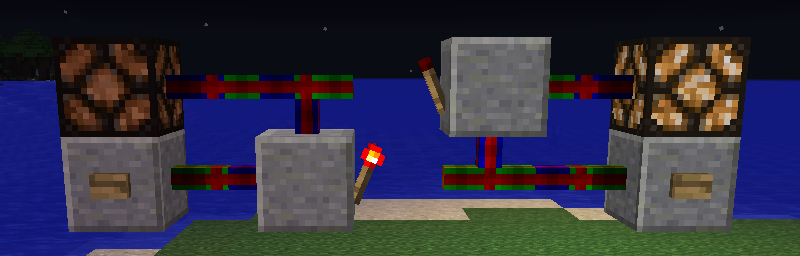
\includegraphics[width=\textwidth]{1_bit_pipes}\\

\subsection{32-bit Signal Wire}
\bf 32-bit Signal Wires \rm support full integer range and work a bit different:
Here you can set each side of each block individually to be either input(blue), output(green), both(cyan) or none(not connected), right-click with empty hand to cycle. The output signal for all outputs is calculated by combining all input signals on the whole connected wire system via bitwise OR operation.

It's recommended to not connect a wire to itself via input and output or two wires to each other via bidirectional connection because you would end up with self-sustaining redstone signals.

\section{Signal components}
\subsection{8-bit Lever}
The \bf 8-bit lever \rm provides redstone signals in range $000\dots255$. It has a front side with 8 red switches that binary encode the block's output signal. The upper row encodes 1 2 4 8 and the lower row 16 32 64 128. Each lever can be flipped by simple right click, down is off and up is on.

\subsection{Signal LED-display}
The \bf Signal LED-display \rm displays the redstone signal it is receiving. When right clicked it will open its GUI that allows detailed configuration about how to display:
Signal bit offset and signal size define which bits of the input signal should be used to encode the number. Leave them at 0 32 to use all bits, unless you are transmitting multiple separate numbers within one signal. Numbers can be displayed in either decimal (normal) or hexadecimal (base 16) mode using the format string or in binary mode as 8 lamps that are oriented the same like in the 8-bit Lever.
The two text fields on top and bottom are for description texts that will be shown above and below the number.
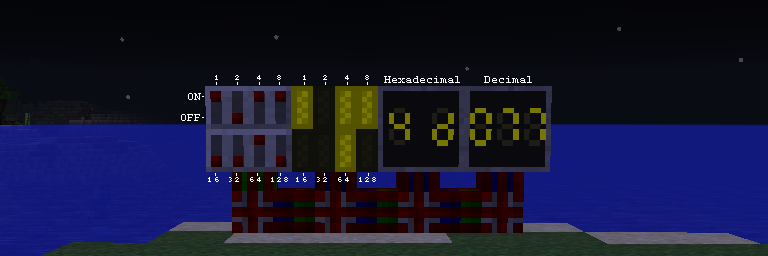
\includegraphics[width=\textwidth]{8_bit_io}\\

\section{Inventory control}
\subsection{Inventory connectors}
\subsection{Inventory reader}
\subsection{Item translocator}
\it Documentation coming soon!\rm

\section{Integerated redstone circuits}
\imgtex

\includegraphics[align = t]{circuit} & The \bf Redstone Circuit \rm block allows you to put complicated redstone logic circuits into one single block, making them very compact and a bit cheaper in redstone cost. To define what the block should do you need to program it using the \bf Circuit Programmer \rm (explained later).\\
\end{tabularx}

\subsection{Creating \& using a circuit}
\imgtex

\includegraphics[align = t]{assembler} & Also your circuit needs some logic gates, IO-ports, and counter to perform the program. These are installed using the \bf Circuit Assembler\rm .
The exact amount of these parts depend on your program and is displayed in the Circuit Programmer when trying to put the program on the circuit.\\
\end{tabularx}

For creating circuits in the assembler put the citcuit item into the top right slot. Adding logic gates requires 1 redstone dust each, adding counters requires 2 netherquartz each and adding available signal outputs requires 1 lever each. Put the ingredients into the 3 left slots and click on the big button int the middle to insert them. Circuits can also be disassembled again on the left side of the assembler's GUI giving you the parts back. The circuit's internal logic can contain up to 128 gates and/or up to 8 8-bit counter and up to 16 outputs.\\
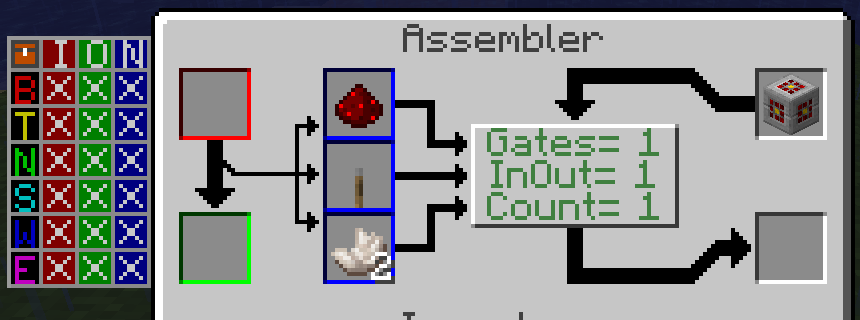
\includegraphics[width = \textwidth]{assembler_gui}\\
\it About the colored tab on the very left read section 2.1 "Machine Configuration" in the Inductive Automation Manual. \rm\\

When placed, the circuit block has 16 1-bit channels for each input and output, so to use all of them with only 6 available block faces, you would need to use 8-bit wire or place multiple circuits next to each other. Therefore they are bundled into four 8-bit chunks (2 in + 2 out).

In the circuits's GUI you can set for each block face, which 8-bit chunk to use and a HEX-AND-gate filter that should be applied (like in \bf logic signal converter\rm ). So applying a normal redstone signal will set all bits contained in the filter to on and for output a redstone signal will be emitted if at least one of the bits contained in the filter is on.

The circuit's internal logic does the following:
The state of all gates is updated each operation tick, based on the individually defined input states and the type of logic operation they represent. This is done in the order they appear in the programm using the input states present at that time, so referring to previous gates will use their just updated state and referring to later gates (or themself) will use the state they had after last update tick.

After that the counters will count up by one if the gate defined as SET-input is on, otherwise if the gate defined as RESET-input is on they will go back to 0. They also go back to 0 if they reach above 255. Their current 8-bit counting states are stored in gate slots $64\dots127$ using 8 for each counter, so when using counters these slots are occupied and can't be used for logic gates.

Finally the circuit's outputs will be set to the state of the individual gates they are bound to.

The operation tick interval can be set in the circuit's GUI. It also contains a ON/OFF button to run or pause updating and a RESET button to set all gates to off.

\subsection{Programming}
To actually tell the circuit what it should do, you need to apply a program to it in the \bf Circuit Programmer\rm :\\
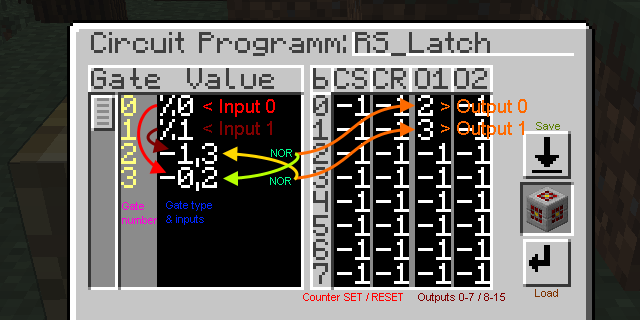
\includegraphics[width = \textwidth]{programmer_gui}\\
\it This shows it's GUI with a RS-Latch setup as example. The colored arrows and texts are edited to illustrate the signal flow. \rm\\
Gates are defined on the left part of the GUI with the following syntax. Each line defines one gate and has to start with one character representing it's type and is directly (no whitespace) followed by its parameters. 

For logic gates the parameters are the gate numbers that should be used as input, separated by colons ',' (also no whitespace). For redstone input it's the number of the circuit's input channel that this gate should be set to. And for the 8-bit comparator it's the number of the 8-bit chunk of gates (= number of it's first contained gate divided by 8), whose numerical representation should be compared, followed by the comparator character, followed by a decimal number in range 0-255 to compare with. All currently available gate types are listed in this table:\\
\begin{tabular}{|c|c|l|l|} \hline
\bf Type & \bf Ch & \bf Parameters & \bf Function \\\hline
RS input & $\%$ & input channel & Active if channel receives redstone signal \\\hline
OR gate & $+$ & 0-15 inputs & Active if any input active, otherwise inactive \\\hline
NOR gate & $-$ & 0-15 inputs & Inactive if any input active, otherwise active \\\hline
AND gate & $\&$ & 0-15 inputs & Inactive if any input inactive, otherwise active \\\hline
NAND gate & $*$ & 0-15 inputs & Active if any input inactive, otherwise inactive \\\hline
XOR gate & $/$ & 0-15 inputs & Active if uneven number of inputs active \\\hline
XNOR gate & $\backslash$ & 0-15 inputs & Active if even number of inputs active \\\hline
8-bit Comp. & $\#$ & input$=$number & Active if 8-bit input equal to number \\\hline
8-bit Comp. & $\#$ & input$<$number & Active if 8-bit input smaller than number \\\hline
8-bit Comp. & $\#$ & input$>$number & Active if 8-bit input greater than number \\\hline
\end{tabular}\\

The up to 8 counters of the circuit are defined in the columns on the right marked with 'CS' and 'CR'. The 'CS' (Counter SET) column gets the gate number that need to be active for the individual counter to count up by one. And the 'CR' (Counter RESET) column gets the gate number that needs to be active to set the counter back to zero. If reset gate is set to '$-1$' the counter will only go back to zero if it reaches an 8-bit integer overflow ($>255$). Set both values to '$-1$' for counters you don't use (every counter costs 2 netherquartz).

As already mentioned before each counter occupies 8 gates to store its value, where counter 1 uses gates $64-71$, counter 2 uses $72-79$ and so on ($64 + counterId * 8$). These gates can be referenced in the program like any other gate, but the most common way is to use the 8-bit compare gate to check if the counter value is below, above or equal to a certain number. In this case the 8-bit chunk number for the comparator gate is simply the counter  number plus 8.\\

And the last two columns marked with 'O1' and 'O2' define which gate should be used for which output channel, where 'O1' defines channels $0-7$ and 'O2' defines channels $8-15$. Set outputs to '-1' if you're not using them (every output costs a lever).\\

To put your settings onto a circuit, just give it a name in the line on top, put the circuit into the only available slot and click the save button. If everything is fine you should get a "Compiling successful" message and the tooltip of the circuit should show the program name you have set. If your gate definitions contain errors you get a message that tells "Compile error" with the line that was wrong. Otherwise if your circuit is missing gates, counter or outputs required to execute your settings you get a message that tells you what is missing.

To store your settings for later use you can also save it on a piece of paper and later load it into the programmer again by clicking the load button. If you don't need a circuit program anymore just put the item into the crafting grid to get the paper back.

\subsection{Example programms}
A \bf timer \rm that emits a 1 tick redstone signal every 150 ticks and resets if receiving a signal:
\begin{lstlisting}
Gates:
0: %0		get input signal
1: #8=149	check if counter reached 149
2: +0,1		reset counter if it reached 149 or input active
3: -0		increase counter if input not active
Counter 0: CS=3 CR=2
Outputs: 1	emit signal if counter reached 149
Total cost: 4 redstone dust, 2 netherquartz, 1 lever
\end{lstlisting}
A \bf clock \rm that displays time in minutes and seconds on two 8-bit Displays. Input signal on channel 0 lets the clock run and signal on channel 1 resets it. (Circuit tick interval must be set to 0.05s):
\begin{lstlisting}
Gates:
0: %0		get run signal
1: %1		get reset signal
2: #8=19	check if 19 ticks have passed
3: #9=59	check if 59 seconds have passed
4: &2,3		reset second counter after 59.95s
5: +1,4		or if receiving reset signal
6: +1,2		reset tick counter after 19 ticks or reset signal
Counter 0: CS=0 CR=6	counting ticks
Counter 1: CS=2 CR=5	counting seconds
Counter 2: CS=4 CR=1	counting minutes
Outputs: 
72 - 77		to display seconds (6-bit)
80 - 87		to display minutes (8-bit)
Total cost: 7 redstone dust, 6 netherquartz, 14 lever
\end{lstlisting}

\it there will be probably added more in the future \rm

\end{document}